\chapter{Il linguaggio per l'orchestrazione}

Abbiamo visto come SOA e i Servizi Web siano una delle risposte più recenti
alla necessità di integrare funzionalità applicative eterogenee, e di fornire
un modello di sviluppo software che sia il pi\`u efficace possibile rispetto
alla natura dinamica dei domini applicativi tipici delle grandi realtà
aziendali.

Alla base della metodologia SOA vi è l'approccio ``bottom-up'', secondo cui è
possibile comporre le funzionalita di base offerte dalle diverse applicazioni
aziendali per crearne di più complesse e articolate. Gli standard e i linguaggi
dei Web Services foniscono il supporto tecnologico e formale per realizzare tale
integrazione che nella maggior parte degli scenari reali prevede di dover far
comunicare tecnolgie e formalismi del tutto eterogeni e incopatibli. Uno delle
possibilità più interessanti è quella di poter utilizzare il patrimonio storico
(``legacy'') del software azzindale tramite standard moderni e aperti, e poter
fare dialogare le applicazioni di ultima generazione con quelle più ``mature'',
che spesso mantengono un alto valore aziendale ma si basano su tecnologie e
metodologie proprietarie ormai difficilmente manutenibili.

Predisporre i componenti e renderli disponibili secondo il paradigma della
Architettura Orientata ai Servizi certo non realizza tutte le necessità di un
complesso sistema aziendale, il passo successivo non può essere che quello di
comporre le singole funzionalità di base per realizare i flussi operativi che
implemetano le reali politiche e strategie di business. Le attività aziendali
quindi possono essere rappresentate come processi (``Business Process'') che
raggruppano le singole funzionalità secondo precise regole aziendali (``Business
Rules'') e tramite primitive di aggregazione che attuano dipendeze temporali e
logiche fra i diversi componenti publicati come servizi (``Service
Orchestration''). Se si può pensare che le singole funzionalità siano i mattoni
del business e che abbiano una certa robustezza temporale, in termini di
specifica e implemetazione, i processi al contrario possono essere fortemente
dinamici e mutevoli, per poter facilmente adeguarsi alle necessità sempre nuove
che si presentano nelle attività di un'azienda.

Si capisce quindi come nasca la necessità di un formalismo specifico per la
definizione e realizzazione di tali processi. In generale si vorrebe poter
disporre di un linguaggio semplice e flessibile che possa essere utilizzato a
diversi livelli aziandali, compreso e adoperato dalle diverse figure
professionali che partecipano alla definizione e attuazione dei processi
stessi. Si vorrebbe disporre non solo di un linguaggio di programmazione
utile ai tecnici del software ma anche di un formalsmo usabile dai manager e
dagli esperti dei domini applicativi, che potese realizzare una piattaforma comune
per la collaborazione fra le diverse arie disciplinari.

E' proprio come risposta a tale necessità che si propone BPEL, un linguaggio
basato su XML per la definizione di processi aziendali realizzati come
composizione di funzionalità esposte da Servizi Web. BPEL storicamente nasce
dalla fusione di due teconlogie sviluppate indipendetemente all'inizio degli
anni 2000: WSFL (Web Service Flow Language) di IBM e XLANG di Microsoft. La
prima versione del linguaggio (BPEL4WS ``Business Process Execution Language for Web Services - Version 1.0'')
risale al 31 Luglio 2002 e fu prodotta del lavoro congiuto di grandi
aziende come IBM, BEA, SAP, Siebel e Microsoft. Dall'Aprile del 2003 il lavoro
di stesura della versione successiva (1.1) è stato affidato alla supervisione di
OASIS, società nata con il compito di realizzare standard aperti e condivisi
dalla comunità internazionale, al 5 Maggio 2003 è datato il rilascio di questa
versione nella stesura ufficiale. Oasis è  anche la curatrice della
versione 2.0 dello standard (WS-BPEL ``Web Services Business Process Execution
Language Version 2.0'') che ha visto il primo rilascio ufficiale in data
11 Aprile 2007.
\\
\ldots
\newpage

Nonostante BPEL sia ampiamente documentato da specifiche e standard ufficiali e
sia disponibile in diverse implemetazioni, le problematiche realitive al suo
uso non mancano e alcune di esse possono essere attribuite alla
mancanza di una semantica formale. Il processo di realizzazione di applicazioni BPEL
risulta difficile e fortemente soggetto ad errori anche per la presenza di
costrutti complessi come: il parallelismo, la concorrenza, la terminazione
forzata di attività, la correlazione e la compensazione, quest'ultima utilizzata
per la realizzazione di ``Long-Running Transaction'', e forse ancora non 
compresi in tutti i lori aspetti e potenzialità dagli utilizzatori. In tal
senso si è pensato che un processo di analisi e di formalizzazione di
tali costrutti potesse essere utile sia per chi si trova ad utilizzarli sia per
coloro che ne definiscono le specifiche in linguaggio naturale.

Un approccio, per cercare di affrontare queste problematiche, è stato quello di
utilizzare la teoria dei metodi formali e delle algebre di processo per la
definizione di una sematica formale e per la realizzazione successiva di una
piattaforma per la verifica e la dimostrazione di proprietà di applicazioni
basate su BPEL. Con tale scopo è stato creato Blite, una variante semplificata di
BPEL, che riproduce alcune delle sue funzionalità più caratteristiche cercando
d'altra parte di semplificarne alcuni aspetti ritenuti marginali nella
realizzazione del modello Process Orinted.
   
Il lavoro svolto in questa tesi è da considerarsi a supporto di questa attività,
come un ulteriore verifica e confronto del processo di astrazione teorica e
formale con gli aspetti più concreti e tecnologici legati all'implementazione di
un linguaggio come BPEL per l'orchestrazione distribuita di servizi. Infatti
l'obiettivo primario è stato quello di realizzare un'implemetazione di Blite che
potesse essere il più vicino possibile, per caratteristiche e applicabilità, ai
motori di esecuzione di BPEL attualmente disponibili. Se da un lato Blite vuole
essere un'analisi di BPEL fatta tramite un processo di astrazione e
formalizzazione, il lavoro qui esposto vuole essere a sua volta un'analisi di
tale processo, nel senso che ne vuole verificare la compatibilità e l'attinenza
con le problematiche più concrete e tecnologiche presenti nell'ambito della
orchestrazione di servizi. Di fatto quello che abbiamo fatto non è altro che un
test critico di come i costrutti formali utilizzati per fornire la semtica del
liguaggio, potessero essere realmente implementati in scenari di sowfware di
produzione, che quindi continuassero a mantenere un legame a doppio filo con il
mondo delle tacnologia da cui hanno tratto iniziale ispirazione.
\\

Di seguito andremo a decrivere la sintassi e  la sematica originali di Blite e
le versioni leggermente modificate di cui è stata realizzata l'implementazione.

%%%%%%%%%%%%%%%%%%%%%%%%%%%%%%%%%%%%%%%%%%%%%%%%%%%%%%%%%%%%%%%%%%%%%%%%%%%%%%%%
% BLITE
%%%%%%%%%%%%%%%%%%%%%%%%%%%%%%%%%%%%%%%%%%%%%%%%%%%%%%%%%%%%%%%%%%%%%%%%%%%%%%%%
\section{Blite, un approccio formale a BPEL}

Come già detto Blite è un linguaggio che può essere visto come una
semplificazione di BPEL, nel senso che ne ripropone solo alcuni aspetti
essenziali come: partner links, process e activity termination, message
correlation, fault handler e compesation handler, mentre ne tralascia altri,
sepur interessanti, come timeout, eventi, termination handler e flow graph. 

Anche il modello di invocazione dei servizi è stato semplificato. In BPEL difatti
sono possibili sia invocazioni one-way che request-response. Le prime sono
invocazioni asincrone, in cui il clinet dopo aver invocato può continuare la sua
elaborazione senza dover attendere alcuna risposta, le seconde invece realizzano
invocazioni sincrone, in cui l'operazione di richiesta blocca il client fino al
sopraggiungere del risultato. In Blite è stato di fatto scelto di supportare
solamente la comunicazione asincrona, in qualto il comportamento sincrono può
essere sempre riprodotto tramite l'opprtuna sequenzializzazione di operazioni
asincrone.
% In pratica in BPEL sono presenti le tre primitive di comunicazione
% \texttt{invoke}, \texttt{receive} e \texttt{replay}, in Blite rimangono
% solamente la \texttt{invoke} e la \texttt{receive}

Anche il meccanismo di instradamento dei messaggi alle opprtune istanze di
processo è stato semplificato. In generale in BPEL tale obiettivo può essere
realizzato con due tecniche alternative: il \emph{WS-Addressing}, che guida
l'indirizzamento in base al valore di meta infomazioni
contenute negli header, e la \emph{Correlazione (Message
Correlation)} che invece discrimina rispetto ai valori applicativi contenuti in
determinate parti del corpo stesso dei messaggi. I Blite è stato scelto di
rappresentare solamente quest'ultima metodologia.

La sintassi di Blite è data in Tabella \ref{tab:syntaxwsbpel}. La categoria
sintattica \emph{Servizio (Service)} rappresenta  sia la definizione di
processo $\xproc{\xsa}{\xh_f}$, che le istanze nella loro esecuzione a runtime
con uno specifico stato della memeoria, $\xinst{\xsigma}{\xs}$; quest'ultima
forma non specifica ulteriormente il linguaggio ma serve per poter introdurre
una rappresentazione della fase di esecuzione indispensabile per
poter definire la sematica operazionale.

Una definizione di servizio è semplicemente uno \emph{Scope} (o
\emph{Contesto}) in cui è definita una
\emph{Start Activity} $\xsa$ e un \emph{Fault Handler} $\xh_f$. Difatti si
impone che le attività iniziali di un processo siano un sott'insieme di tutte
quelle possibili e che in pratica la prima attività operativa (o \emph{Basic
Activity}) sia una ricezione. Le attività infatti sono divise in due categorie
principali, le \emph{Basic Activity} e le \emph{Structured activities}. Le
prime sono l'attività primitive, cioè individuano le operazioni di
base compiute da un'istanza di processo, le seconde sono una composizione
strutturale di quest'ultime. Di fatto le attività di base sono costituite
dalla invocazione asincrona $\xinv{\plinv}{\xo}{\bar{\xx}}$ di un'operazione
remota $\xo$ su un \emph{partner link} $\plinv$ con parametri attuali
$\bar{\xx}$, dall'attesa dell'invocazione $\xrec{\plrec}{\xo}{\bar{\xx}}$
dell'operazione locale $\xo$ tramite il \emph{partner link} $\plrec$ con
parametri formali ${\bar{\xx}}$, dall'assegnazione della valutazione
dell'espressione $\xe$ alla variabile $\xx$, dalla attività vuota $\xskip$,
dalla sollevazione di una eccezione $\xthr$ e dalla operazione di terminazione
d'istanza $\xexit$.

%%%%%%%%%%%%%%%%%%%%%%%% SYNTAX TABLE %%%%%%%%%%%%%%%%%%%%%%%%%%%%%%%
\begin{table}[t]
\begin{small}
$$
\delimite{
\begin{array}{
@{\hspace{-1ex}}l@{\hspace{2ex}}r@{\hspace{.75ex}}l@{\!}l@{\hspace{3ex}}l@{\hspace{-1ex}}}
\textit{Basic activities} & \xa & ::= &
\xinv{\plinv}{\xo}{\bar{\xx}} \!\sepgr\!
\xrec{\plrec}{\xo}{\bar{\xx}} \!\sepgr\!
\xass{\xx}{\xe} & \textrm{invoke, receive, assign}\\[-.05cm]
 &  & \!\sepgr\! &
\xskip \!\sepgr\!
\xthr \!\sepgr\!
\xexit & \textrm{empty, throw, exit}\\[0.25cm]
%
\textit{Structured activities} & \xs & ::= &
\xa \!\sepgr\!
%\xif{\xx}{\xs_1}{\xs_2} \!\sepgr\!
\xif{\xe}{\xs_1}{\xs_2} \!\sepgr\!
%\xwhile{\xx}{\xs} & \textrm{basic, conditional, iteration}\\
\xwhile{\xe}{\xs} & \textrm{basic, conditional, iteration}\\[-.05cm]
& & \sepgr & \xs_1\xsucc\xs_2 \sepgr
\sum_{j \in J}\xrec{\plrec_j}{\xo_j}{\bar{\xx}_j}\recsep\xs_j &
\textrm{sequence, pick (with $\length{J} \,> 1$)}\\[-.05cm] & & \sepgr & \xs_1
\xpar\, \xs_2 \sepgr \xscopefc{\xs}{\xh_f}{\xh_c} & \textrm{parallel, scope}
\\[0.25cm]
%
\textit{Start activities} & \xsa & ::= &
\xrec{\plrec}{\xo}{\bar{\xx}} \!\sepgr\!
\sum_{j\in J}\xrec{\plrec_j}{\xo_j}{\bar{\xx}_j}\recsep\xs_j & \textrm{receive,
pick}\\[-.05cm] & & \sepgr & \xsa \xsucc \xs \!\sepgr\! \xsa_1 \xpar\, \xsa_2
\sepgr \xscopefc{\xsa}{\xh_f}{\xh_c} & \textrm{sequence, parallel,
scope}\\[0.25cm]
%
\textit{Services} & \xI & ::= &
\xproc{\xsa}{\xh_f} \sepgr
\xinst{\xsigma}{\xs} \sepgr
\xinst{\xsigma}{\xs} \xmid \xI & \textrm{definition, instance,
multiset}\\[0.25cm]
%
\textit{Deployments} & \xd & ::= &
\xeng{\xI}{\xcorr} \sepgr
\xd_1 \xspar \xd_2 &  \textrm{deployment, composition}
\end{array}
}
$$
\end{small}
  \vspace*{-1.20cm}
  \caption{La sintassi di Blite}
  \label{tab:syntaxwsbpel}
  \vspace*{-0.3cm}
\end{table}
%%%%%%%%%%%%%%%%%%%%%%%% FINE TABLE %%%%%%%%%%%%%%%%%%%%%%%%%%%%%%%

Le attività strutturate sono costituite invece dalla scelta condizionale
$\xif{\cdot}{\cdot}{\cdot}$, dalla iterazione $\xwhile{\xe}{\xs}$, dalla
composizione sequelziale di sottoattività $\xs_1\xsucc\xs_2$, dalla scelta
esterna su un set non vuoto di possibili porte $\sum_{j \in
J}\xrec{\plrec_j}{\xo_j}{\bar{\xx}_j}\recsep\xs_j$\footnote{La scelta può
essere anche espressa tramite l'operatore binario $ \cdot + \cdot$.}, dalla
composizione parallela di attività $\xs_1\xpar\, \xs_2$ e per finire dal costrutto di scope o contesto $\xscopefc{\xs}{\xh_f}{\xh_c}$, dove ad una attività pricipale
detta \emph{Contest Activity} $\xs$ viene associato un \emph{Fault Handler}
$\xh_f$ e un \emph{Compensation Handler} $\xh_c$.

La sintassi afferma che le operazioni di comunicazione siano
definite su i partners link $\plinv$ per l'invocazione e $\plrec$ per la
recezione. Un ulteriore imposizione viene fatta sulla struttura sintattica di
tali oggetti richiedendo che essi siano tuple di uno o al massimo due elementi,
con la seguente ulteriore restrizione

$$
\begin{array}{ccc}

\plinv = \left\{ 
\begin{array}{l}
 \arr{\xu,\xp}   \\
 \arr{\xu}  
\end{array} \right.

&

\plrec = \left\{ 
\begin{array}{l}
 \arr{\xp,\xu}   \\
 \arr{\xp}  
\end{array} \right.

& \textrm{con } \xp \textrm{ staticamente noto e } \xu \textrm{
evetualemente variabile}

\end{array}
$$

Di fatto i partner link possono essere mono direzzionali $\arr{\cdot}$ o
bidirezionali $\arr{s1, s2}$. In quest'ultimo caso sottindendono una
comunicazione asincrona richiesta-risposta, secondo cui ad una invocazione sul servizio $s1$
quest'ultimo risponderà in maniera asincrona con una risposta sul servizio $s2$.
Di fatto si impone anche che i nomi dei servizi su cui si eseguono le ricezioni
siano staticamente noti\footnote{Quest'ultima imposizione rispecchia il
fatto che staticamente sono noti i contratti e fissate le
locazioni su cui essi sono disponibili; a runtime le varie istanze si possono
scambiare quest'ultima informazione, ma il modello non prevede che possano
nascere ne nuovi contratti ne nuove locazioni dove questi siano implementati.}.
Un esempio di comunicazione asincrona con i costrutti definiti da Blite è
rappresentato in Figura \ref{fig:lin:com}, dove è esplicitato il fatto che i
nomi dei servizi $s1$ e $s2$ oggetto delle invocazioni sono determinati a
runtime.

\begin{figure}[ht]
\begin{center}
  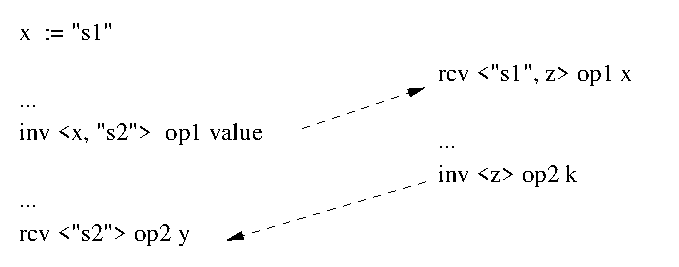
\includegraphics{linguaggio/dia/com}
   \caption[Comunicazione asincrona con Blite]{
   	\textsf{{\small Realizzazione della comunicazione asincrona
   	richiesta-risposta con i construtti della sintassi di Blite}} }
  \label{fig:lin:com}
\end{center}
\end{figure}

La composizione distribuita di diversi processi viene definata dalla categoria
sintattica \emph{Deployments}. Il termine $\xd_1 \xspar \xd_2$ rappresenta la
contemporanea escuzione di tutte le istanze ottenute dalle
definizioni presenti in $\xd_1$ con quelle di $\xd_2$. Il \emph{Deployment}
$\xeng{\xI}{\xcorr}$ è la definizione di processo $\xI$ con tutte le sue attuali
istanze a cui è stato associato il \emph{Correlation Set} $\xcorr$. Tale insime
individua fra tutte le variabili presenti nella definizione del processo quelle
che dovranno essere considerate per valutare la correlazione di un messaggio
rispetto alla diverse istanze. Vedremo come la sematica di Blite definisca tale
processo di attribuzione di un messaggio a una particolare istanza e come tale
sematica sia stata implemetata nel nostro engine di esecuzione.
 
In generale si impone la restrizione che un insieme di deployments sia
\emph{ben formato}, nel senso che i nomi nei partner link utilizzati per le
ricezioni non siano condivisi fra diversi deployment. In questo modo ogni
definizione di processo avrà i propri nomi di servizo univoci e dato un nome
sarà sempre possibile individuare un deployment preciso.
\\

Per concludere si deve osservare come la sintassi esposta debba essere ancora
considerata ``astratta'' in quanto non definisce tutti gli aspetti necessari
all'imlemetazione. In particolar modo non definisce i tipi dei valori
attribuibili alle variabili, ne la sintassi delle espressioni supportata, e
nemmeno esplicita la precedenza degli operatori di sequenzializzazione,
parallelismo e scelta esterna\footnote{In merito alla precedenza degli
operatori, il documento originale in cui è descritto Blite, afferma che
l'operatore di sequenza $\cdot ; \cdot$ ha precedenza
sull'operatore di parallelismo $\cdot | \cdot$, e questo ha precedeza
sull'operatore di scelta $\cdot + \cdot$}. Di fatto l'implemetazione da noi
realizzata fa riferimento ad una sintassi concreta che definisce in maniera
formale anche questi aspetti. In particolare vedremo come  i semplici
operatori binari siano trasformati in costrutti con 
delimitatori di blocco. In questo modo risulta più semplice
l'implementazione del parser, in quanto evita la necessità di eseguire
\emph{lookahead}, e anche la precedenta di un attività rispetto l'altra risulta
esplicitata nalla codifica stessa dei blocchi. In questo modo il codice risulta
più leggibile e più simile nella struttura ai tradizionali linguaggi di
programmazione.
